\section{Introduction}
\label{sec:intro}

A traffic classifier that reports 97\% accuracy on a benchmark has told you
almost nothing about what is achievable on your network. It has not told you
whether 99\% is reachable with a longer observation window, whether 97\% is
already at the limit the channel permits, or whether the remaining 3\% is
irreducible for reasons that have nothing to do with the classifier. Detectors
in this area are evaluated by their own error rates, and an error rate is a
statement about one system rather than a statement about the problem.

What a practitioner needs is the other direction: a bound on how well
\emph{any} classifier can do, at a stated observation window, for a stated pair
of services. The ingredients for that exist, but they share a limitation that
matters here. Classical work gives feature-conditional bounds for closed-set
fingerprinting, and recent work establishes that side-channel leakage is
inevitable under explicit conditions and characterizes a rate-distortion
frontier for defense. Both are single-letter or i.i.d.-conditional: exponential
error decay requires repeated conditionally independent observations, and the
frontier is proved inside a stationary-memoryless class. Real packet prefixes
are neither independent nor stationary, and the gap between what those results
assume and what a trace provides is exactly the gap a practitioner must cross.

We call the resulting object \emph{certification-grade}: every number it reports
is tied to a stated confidence level and a stated assumption, each named rather
than borrowing strength from the other.

We measure a two-sided indistinguishability bracket on real encrypted traffic
instead, and we give each side a confidence level rather than pairing a proven
side with an unproven one. The upper side is a finite-sample bound on the total
variation distance between two services' prefix laws, with a radius whose two
terms we derive explicitly. The lower side is a classifier-based bound at a
nominal confidence level, distribution-free in the same sense. The two sides
differ in construction and in tightness, not in whether a guarantee is
available: the upper radius is fixed by the alphabet and the flow counts, while
the lower bound must hold against an adversarial choice of decision function and
is correspondingly wider. It is the upper side that an error-floor claim needs
and the upper side that in practice binds, which is a statement about this
construction rather than about what is provable.

The bracket is computable, and it is computable at a resolution that is
deliberately coarse. On the CESNET-QUICEXT-25 XS subset, at the coarsest channel
we pre-register, 336 of 990 service pairs (33.9\%) admit an interval whose upper
side is finite-sample strict and whose lower side clears the gate
(\Cref{tab:bracket}). \Cref{fig:bracket} shows the measurement end to end: raw
flow records are quantized into a prefix symbol, the symbol feeds an upper and a
lower branch that carry different certification strength, and the two branches
meet only at the gate. The certificate is not free: raising the alphabet
resolution makes the channel more informative and destroys the certificate at
the same time, because the confidence radius grows with the alphabet size while
the threshold does not. The upper-side set falls from 340 pairs at the coarsest rung
to none four rungs finer, and the joint gate admits 336 at that rung because four
pairs clear the upper side and fail the lower (\Cref{fig:horizon}). The coarse
channel is therefore not a concession to tractability but the only regime in
which a two-sided certificate exists at these prefix lengths and flow counts.

We also report a negative result that we consider part of the contribution. The
natural estimator for how divergence accumulates across dependent packet
positions is a chain-rule plug-in, and it cannot answer the question on this
data. On a synthetic source whose analytic per-position divergence is known
exactly, the estimator returns sublinear growth, deflating its estimate to
$0.6769$ of the truth on the plain arm at the longest prefix
(\Cref{fig:estimator}). The cause is measured rather than conjectured: prefix
occupancy collapses as the prefix lengthens, and a per-position smoothing bias
accumulates exactly where contexts are sparse. Two independent repairs both fail
their known-truth gate, and the repair that would work discards more than half
the data at the upper end of the range. We report this as a methods and limits
finding, not as an estimate of a growth rate, and the question is left open with
the reason stated in numbers.

\paragraph{Contributions.}
\begin{itemize}
  \item \textbf{A pairwise indistinguishability certificate on real encrypted
  traffic.} We compute a per-pair interval whose upper side is a finite-sample
  bound and whose lower side is a classifier-based bound at a nominal confidence
  level, measured over all 990 pairs at the coarsest pre-registered channel
  (\Cref{sec:design}, \Cref{sec:results/bracket}). 33.9\% of pairs satisfy the
  joint gate, and at that rung the upper side is the scarce object. The
  certified object is the pair: its content is the two-point bound on a test
  between those two services, and we make no multi-class claim.
  \item \textbf{The certificate horizon, as a function rather than a number.}
  We show that a finer alphabet resolves more and certifies less, that the
  upper-side set is empty at and beyond the fourth rung, and that the boundary has a
  closed form in resolution, sample size, and distance whose two derivation
  routes agree to zero (\Cref{sec:results/horizon}). Where the certificate is
  lost, a conditional divisibility bound keeps the large-prefix regime
  non-empty.
  \item \textbf{A methods and limits finding for the growth question.} The
  standard chain-rule estimator cannot adjudicate whether divergence grows
  sublinearly here: its bias manufactures the effect it is meant to detect, and
  the failure is robust to two independent repairs at a quantified data cost
  (\Cref{sec:results/estimator}).
  \item \textbf{Bracket validation against real detectors and an independent
  corpus.} On the informative stratum the panel's floor-violation rates fall
  below the null rate, so no detector breaches the certified floor
  (\Cref{sec:results/detector_validation}). The lower side reproduces across
  corpora; the joint gate does not, and the difference is not statistically
  resolved at matched evidence (\Cref{sec:discussion/robustness}).
  \item \textbf{A confound that blocks the obvious corroboration.} A
  heterogeneous-i.i.d.\ null, in which every flow draws its own rate and then
  emits independent bits, reproduces the first-order-Markov vote that would
  otherwise look like evidence of within-flow dependence; the vote is therefore
  not diagnostic (\Cref{sec:results/estimator}).
  \item \textbf{Two further measured quantities that bound the scope.} A second
  certified object over whole-flow rectified statistics is reported alongside the
  prefix law, and its agreement with it is cancellation rather than
  corroboration, so the two may not be ranked (\Cref{sec:discussion/objects}).
  The unknown-class mass a bracket omits is estimated as a deployment-site
  quantity rather than a universal prior (\Cref{sec:discussion/missing_mass}).
\end{itemize}

\paragraph{Novelty boundary.} To our knowledge, no prior work measures a
two-sided bracket with asymmetric guarantee strength on real encrypted traffic,
where the asymmetry is one of constant provenance and confidence-level kind
rather than provenness; \Cref{sec:related/novelty} gives it in full.

\paragraph{Scope.}
The bracket is a measurement instrument, not a vulnerability. We consume a
(direction, size) channel and no name, address, or content field, and we quantify
what including an identifier would change rather than assuming it is immaterial.
The certified fraction is a stratum statement, and we state the stratum wherever
we quote it.

\begin{figure}[t]
\centering
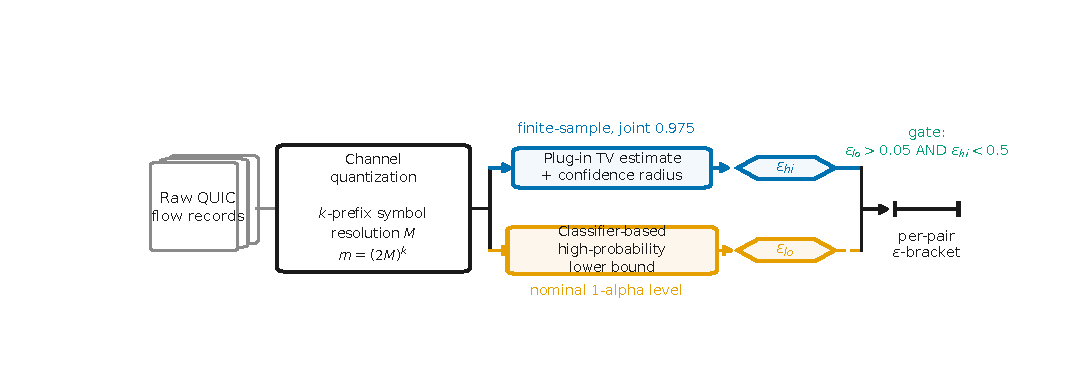
\includegraphics[width=0.86\columnwidth]{figures/paper/fig1_bracket_overview.pdf}
\caption{The EIBO measurement. Raw QUIC flow records are quantized into a
$k$-prefix symbol over a (direction, size) alphabet at resolution $M$. The
quantized symbol feeds two branches that carry different certification
strength: an upper branch combining a plug-in TV estimate with a confidence
radius, which is finite-sample, and a lower branch built from a
classifier-based high-probability lower bound whose constant is asymptotically
derived, so its level is nominal. The
branches meet at the per-pair interval, whose gate is the conjunction
$\epslo > 0.05$ and $\epshi < 0.5$.}
\label{fig:bracket}
\end{figure}
